\input{include/settings.sty}
\input{include/hyphenation.sty}

\title{Python MCU}
\author{Martin Zuther}

\begin{document}

\title{Python MCU}

\subtitle{
  \normalsize{\textrm{\textmd{
        \vfill
        Mackie Host Controller written in Python
        \vfill
        \vspace{10em}
        \vfill
      }}}
}

\author{\normalsize\copyright{} 2011
  \href{http://www.mzuther.de/}{Martin Zuther}}

\date{\normalsize \emph{Last edited on \today}}

\maketitle

\tableofcontents

\clearpage  % layout

\chapter{Mackie Control}
\label{chap:mackie_control}

\textbf{Mackie Control} (abbreviated to MCU), its predecessor
\textbf{Logic Control} and their respective extension units
(\textbf{XT}) are control surfaces that use a proprietary MIDI
protocol to control digital audio workstations (DAWs), especially
their mixing sections.  However, these control surfaces have two
drawbacks: they are definitely not cheap and require quite a bit of
space.  If these are no restrictions to you, by all means go and try
them.

If, on the other hand, you have a certain lack of money or available
space (or you have a controller that is simply too good to be
exchanged for an MCU), you might have found just the application you
need.  It might not support your MIDI hardware controller yet, but if
you know a bit of \textbf{Python} (or a programmer who does) it should
be pretty easy to change that.


\chapter{Installation}
\label{chap:python_mcu}

Download and install the latest version of
\href{http://www.python.org/}{Python 2.6} on your computer.  As of
December 2011, there is no Python 2.6.7 installer for Microsoft
Windows.  Users of this operating system should download
\href{http://www.python.org/download/releases/2.6.6/}{Python 2.6.6},
instead.

Please also download and install these libraries:

\begin{compactitem}
\item \href{http://www.pyside.org//}{PySide} (version 1.0.5 or above)
\item \href{http://www.pygame.org/}{pygame} (version 1.9.1 or above;
  please note that pygame's MIDI implementation is still in its
  infancy and may thus occasionally crash \application{Python MCU})
\end{compactitem}

You'll also need virtual MIDI ports or cables to connect
\application{Python MCU} to your DAW and hardware controller.  I have
successfully used \application{MidiYoke NT} (Microsoft Windows) and
\application{JACK} (GNU/Linux), but others may work just as well.

When you're done, open the directory \path{src} with your file manager
and run the application by double-clicking on the file
\path{PythonMcu.py}.  To get rid of the annoying console window on
Microsoft Windows, try double-clicking on \path{PythonMcu.pyw},
instead.

\chapter{Running Python MCU}
\label{chap:runnint_python_mcu}

Here's a word of warning.  Although I have taken precautionary steps,
there is some inherent risk that your controller might be destroyed by
running \application{Python MCU} (mine was, once, when I was trying to
change a lot of code at once).  So please read the license in
\ref{chap:gpl} before you run \application{Python MCU}, especially the
sections \emph{Disclaimer of Warranty} and \emph{Limitation of
  Liability}.

That being said, here's how to set up \application{Python MCU}\dots

\begin{center}
  \includegraphics[scale=\screenshotscale,clip]{include/images/python_mcu.png}
\end{center}


\begin{description}
\item[Emulation:] Choose between ``Logic Control'' and ``Mackie
  Control''.  The latter should be fine for most current DAWs.  The
  extension units ``Logic Control XT'' and ``Mackie Control XT'' have
  been added for completeness, but I don't think you'll ever need
  them.

\item[Connection:] Determines how \application{Python MCU} connects to
  your DAW.  If you're having trouble with connecting, try changing
  this setting.

  ``Challenge / Response'' forces \application{Python MCU} to register
  with your DAW (which will only work if your DAW supports this),
  whereas ``Wait for MIDI data'' simply waits for some data on the
  MIDI input port.  ``Assume successful connection'' has been added
  for testing purposes -- this setting assumes the presence of a
  Mackie-Control-aware DAW without checking.

\item[MIDI In/Out:] The virtual MIDI cables that connect
  \application{Python MCU} to your DAW.  I freely admit that it's not
  easy to understand the routing of virtual MIDI cables, so I
  recommend using the first cable to send data from
  \application{Python MCU} to your DAW and the second one to send data
  from your DAW to \application{Python MCU}:

  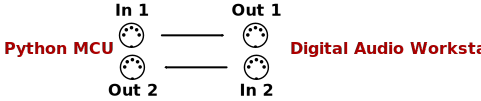
\includegraphics[scale=\screenshotscale,clip]{include/images/virtual_midi_cables.png}

  This way, you can simply look at the screen-shots in this document
  and set up \application{Python MCU} and your DAW accordingly.

\item[Controller:] Select your hardware controller and the MIDI ports
  it provides or is connected to.  There is a text field directly
  below which might give you some hints on connecting your controller
  to \application{Python MCU}.

\end{description}

\chapter{Hardware controllers}
\label{chap:controller_setup}

For the controller assignments of your hardware, please have a look at
\path{doc/Controllers.pdf}.

\section{Novation ZeRO SL MkII}

This adaption makes good use of preset \#32 (Ableton Live Automap), so
you either have to select this preset whenever you want to use
\application{Python MCU} or set it up as your default preset.

Whenever you press the \textbf{Automap} button, \application{Python
  MCU} temporarily stops to let you do your thing in \textbf{Automap}.
When you're done, simply press the \textbf{Automap} button again.

You may also connect a sustain pedal to the ``control pedal'' input
and use it to alternately start and stop playback in your DAW.  If it
doesn't work, you'll have to change the preset: Edit $\rightarrow{}$
Sustain Pedal $\rightarrow{}$ Ports: \textbf{ComnPORT} and MidiChan:
\textbf{ComnCHAN.}  Don't forget to save your changes\dots

\chapter{Digital Audio Workstations}
\label{chap:daw_setup}

\section{Ableton Live}

\begin{description}
\item[Emulation:] Mackie Control (Wait for MIDI data)
\end{description}

\includegraphics[scale=\screenshotscale,clip]{include/images/live_8.png}

\section{Cockos Reaper}

\begin{description}
\item[Emulation:] Mackie Control (Wait for MIDI data)
\end{description}

\includegraphics[scale=\screenshotscale,clip]{include/images/reaper_4.png}

\section{Emagic Logic}

\begin{description}
\item[Emulation:] Logic Control (Challenge / Response)
\end{description}

\includegraphics[scale=\screenshotscale,clip]{include/images/logic_5.png}

\section{Image-Line FL Studio}

\begin{description}
\item[Emulation:] Mackie Control (Wait for MIDI data)
\end{description}

\includegraphics[scale=\screenshotscale,clip]{include/images/fl_studio_10.png}


\chapter{Tested configurations}
\label{chap:tested_configurations}

\section{Hardware controllers}

\begin{compactitem}
\item Novation ZeRO SL MkII
\end{compactitem}

\section{Microsoft Windows XP}

\begin{compactitem}
\item Ableton Live 8
\item Cockos Reaper 4
\item Emagic Logic Platinum 5
\item Image-Line FL Studio Pro 10
\end{compactitem}

\section{Apple Mac}

I haven't got a Mac, but things should work just as well.  Please
report working configurations to me.  Thanks!

\section{GNU/Linux}

\begin{compactitem}
\item ardour 2 (\emph{skipped a lot of commands, though})
\end{compactitem}

\chapter{Extending Python MCU}
\label{chap:extending_python_mcu}

\application{Python MCU} consists of three parts:

\begin{itemize}

\item the \textbf{MackieHostControl} class communicates with a
  connected sequencer using the Mackie Control protocol, translating
  the raw protocol to something much easier to read and use

\item the generalised \textbf{MidiControllerTemplate} class and its
  more specific relatives handle all the details of sending data to
  and receiving data from your hardware controller, again translating
  raw protocols to something easier to read and use

\item finally, the \textbf{McuInterconnector} class connects the
  \textbf{MackieHostControl} and \textbf{MidiControllerTemplate}
  classes (and thus your DAW and hardware controller) with each other

\end{itemize}

This modular design means that the application happily works away with
the irrelevant implementation details being effectively hidden from
you.  As long as you adhere to the internal protocol, you may easily
add your own controller to \application{Python MCU} by deriving a
class from \textbf{MidiControllerTemplate}.

If all this means nothing to you, go find yourself a Python programmer
(or learn Python yourself, it's rather easy and a lot of fun!).  As
long as you know the relevant MIDI implementation of your hardware
controller and worked out a suitable layout of its buttons and
controllers, hooking into \application{Python MCU} is pretty simple.
If you don't believe me, just have a look into the \path{src/Hardware}
directory.

\input{include/gpl_v3.tex}

\end{document}


%%% Local Variables:
%%% mode: latex
%%% mode: outline-minor
%%% TeX-command-default: "Rubber"
%%% TeX-PDF-mode: t
%%% ispell-local-dictionary: "british"
%%% End:
